% This file was converted to LaTeX by Writer2LaTeX ver. 1.0.2
% see http://writer2latex.sourceforge.net for more info
\documentclass{tufte-book}

\usepackage[utf8]{inputenc}
\usepackage[T1]{fontenc}
\usepackage[spanish]{babel}
\usepackage{amsmath}
\usepackage{amssymb,amsfonts,textcomp}
\usepackage{array}
\usepackage{supertabular}
\usepackage{hhline}
\usepackage{graphicx}

\makeatletter
\newcommand\arraybslash{\let\\\@arraycr}
\makeatother
\setlength\tabcolsep{1mm}
\renewcommand\arraystretch{1.3}
\newcommand\wideslash[2]{{}^{#1}/_{#2}}
\newcommand\normalsubformula[1]{\text{\mathversion{normal}$#1$}}
\title{I - INTRODUCCIÓN:}
\author{SOL}
\date{2011-09-01}

\hypersetup{colorlinks}% uncomment this line if you prefer colored hyperlinks (e.g., for onscreen viewing)

%%
% Book metadata
\title{Representaciónes \\ Cartográficas \thanks{Thanks to Edward R.~Tufte for his inspiration.}}
\author[Miguel Starobinsky \ Javier Clavijo]{Miguel Starobinsky \ Javier Clavijo}
\publisher{Publisher of This Book}

%%
% If they're installed, use Bergamo and Chantilly from www.fontsite.com.
% They're clones of Bembo and Gill Sans, respectively.
%\IfFileExists{bergamo.sty}{\usepackage[osf]{bergamo}}{}% Bembo
%\IfFileExists{chantill.sty}{\usepackage{chantill}}{}% Gill Sans

%\usepackage{microtype}

%%
% Just some sample text
\usepackage{lipsum}

%%
% For nicely typeset tabular material
\usepackage{booktabs}

%%
% For graphics / images
\usepackage{graphicx}
\setkeys{Gin}{width=\linewidth,totalheight=\textheight,keepaspectratio}
\graphicspath{{graphics/}}

% The fancyvrb package lets us customize the formatting of verbatim
% environments.  We use a slightly smaller font.
\usepackage{fancyvrb}
\fvset{fontsize=\normalsize}

%%
% Prints argument within hanging parentheses (i.e., parentheses that take
% up no horizontal space).  Useful in tabular environments.
\newcommand{\hangp}[1]{\makebox[0pt][r]{(}#1\makebox[0pt][l]{)}}

%%
% Prints an asterisk that takes up no horizontal space.
% Useful in tabular environments.
\newcommand{\hangstar}{\makebox[0pt][l]{*}}

%%
% Prints a trailing space in a smart way.
\usepackage{xspace}

%%
% Some shortcuts for Tufte's book titles.  The lowercase commands will
% produce the initials of the book title in italics.  The all-caps commands
% will print out the full title of the book in italics.
\newcommand{\vdqi}{\textit{VDQI}\xspace}
\newcommand{\ei}{\textit{EI}\xspace}
\newcommand{\ve}{\textit{VE}\xspace}
\newcommand{\be}{\textit{BE}\xspace}
\newcommand{\VDQI}{\textit{The Visual Display of Quantitative Information}\xspace}
\newcommand{\EI}{\textit{Envisioning Information}\xspace}
\newcommand{\VE}{\textit{Visual Explanations}\xspace}
\newcommand{\BE}{\textit{Beautiful Evidence}\xspace}

\newcommand{\TL}{Tufte-\LaTeX\xspace}

% Prints the month name (e.g., January) and the year (e.g., 2008)
\newcommand{\monthyear}{%
  \ifcase\month\or Enero\or Febrero\or Marzo\or Abril\or Mayo\or Junio\or
  Julio\or Agosto\or Septiembre\or Octubre\or Noviembre\or
  Diciembre\fi\space\number\year
}


% Prints an epigraph and speaker in sans serif, all-caps type.
\newcommand{\openepigraph}[2]{%
  %\sffamily\fontsize{14}{16}\selectfont
  \begin{fullwidth}
  \sffamily\large
  \begin{doublespace}
  \noindent\allcaps{#1}\\% epigraph
  \noindent\allcaps{#2}% author
  \end{doublespace}
  \end{fullwidth}
}

% Inserts a blank page
\newcommand{\blankpage}{\newpage\hbox{}\thispagestyle{empty}\newpage}

\usepackage{units}

% Typesets the font size, leading, and measure in the form of 10/12x26 pc.
\newcommand{\measure}[3]{#1/#2$\times$\unit[#3]{pc}}

% Macros for typesetting the documentation
\newcommand{\hlred}[1]{\textcolor{Maroon}{#1}}% prints in red
\newcommand{\hangleft}[1]{\makebox[0pt][r]{#1}}
\newcommand{\hairsp}{\hspace{1pt}}% hair space
\newcommand{\hquad}{\hskip0.5em\relax}% half quad space
\newcommand{\TODO}{\textcolor{red}{\bf TODO!}\xspace}
\newcommand{\na}{\quad--}% used in tables for N/A cells
\providecommand{\XeLaTeX}{X\lower.5ex\hbox{\kern-0.15em\reflectbox{E}}\kern-0.1em\LaTeX}
\newcommand{\tXeLaTeX}{\XeLaTeX\index{XeLaTeX@\protect\XeLaTeX}}
% \index{\texttt{\textbackslash xyz}@\hangleft{\texttt{\textbackslash}}\texttt{xyz}}
\newcommand{\tuftebs}{\symbol{'134}}% a backslash in tt type in OT1/T1
\newcommand{\doccmdnoindex}[2][]{\texttt{\tuftebs#2}}% command name -- adds backslash automatically (and doesn't add cmd to the index)
\newcommand{\doccmddef}[2][]{%
  \hlred{\texttt{\tuftebs#2}}\label{cmd:#2}%
  \ifthenelse{\isempty{#1}}%
    {% add the command to the index
      \index{#2 command@\protect\hangleft{\texttt{\tuftebs}}\texttt{#2}}% command name
    }%
    {% add the command and package to the index
      \index{#2 command@\protect\hangleft{\texttt{\tuftebs}}\texttt{#2} (\texttt{#1} package)}% command name
      \index{#1 package@\texttt{#1} package}\index{packages!#1@\texttt{#1}}% package name
    }%
}% command name -- adds backslash automatically
\newcommand{\doccmd}[2][]{%
  \texttt{\tuftebs#2}%
  \ifthenelse{\isempty{#1}}%
    {% add the command to the index
      \index{#2 command@\protect\hangleft{\texttt{\tuftebs}}\texttt{#2}}% command name
    }%
    {% add the command and package to the index
      \index{#2 command@\protect\hangleft{\texttt{\tuftebs}}\texttt{#2} (\texttt{#1} package)}% command name
      \index{#1 package@\texttt{#1} package}\index{packages!#1@\texttt{#1}}% package name
    }%
}% command name -- adds backslash automatically
\newcommand{\docopt}[1]{\ensuremath{\langle}\textrm{\textit{#1}}\ensuremath{\rangle}}% optional command argument
\newcommand{\docarg}[1]{\textrm{\textit{#1}}}% (required) command argument
\newenvironment{docspec}{\begin{quotation}\ttfamily\parskip0pt\parindent0pt\ignorespaces}{\end{quotation}}% command specification environment
\newcommand{\docenv}[1]{\texttt{#1}\index{#1 environment@\texttt{#1} environment}\index{environments!#1@\texttt{#1}}}% environment name
\newcommand{\docenvdef}[1]{\hlred{\texttt{#1}}\label{env:#1}\index{#1 environment@\texttt{#1} environment}\index{environments!#1@\texttt{#1}}}% environment name
\newcommand{\docpkg}[1]{\texttt{#1}\index{#1 package@\texttt{#1} package}\index{packages!#1@\texttt{#1}}}% package name
\newcommand{\doccls}[1]{\texttt{#1}}% document class name
\newcommand{\docclsopt}[1]{\texttt{#1}\index{#1 class option@\texttt{#1} class option}\index{class options!#1@\texttt{#1}}}% document class option name
\newcommand{\docclsoptdef}[1]{\hlred{\texttt{#1}}\label{clsopt:#1}\index{#1 class option@\texttt{#1} class option}\index{class options!#1@\texttt{#1}}}% document class option name defined
\newcommand{\docmsg}[2]{\bigskip\begin{fullwidth}\noindent\ttfamily#1\end{fullwidth}\medskip\par\noindent#2}
\newcommand{\docfilehook}[2]{\texttt{#1}\index{file hooks!#2}\index{#1@\texttt{#1}}}
\newcommand{\doccounter}[1]{\texttt{#1}\index{#1 counter@\texttt{#1} counter}}

% Generates the index
\usepackage{makeidx}
\makeindex


\begin{document}

X.- PROYECCIÓN GAUSS-KR\"UGER

La teoría de la proyección conforme del elipsoide terrestre es
establecida por primera vez por el matemático Johann Karl Friedrich
Gauss (1777-1855) entre los a\~nos 1816 y 1827.

\ \ En el a\~no 1821, Gauss aplicó su proyección en trabajos
geodésicos en el estado de Hannover.

\ \ En este sistema la superficie intermedia de proyección en un
cilindro tangente a la largo del meridiano central de la región que
se quiere representar; es apropiado para territorios cuya dirección
de máxima amplitud es en el sentido de las latitudes.

\ \ Las deformaciones dependen solamente del apartamiento del meridiano
central y son simétricas respecto del mismo.

\ \ Cuando se trata de representar territorios muy extendidos en el
sentido de las longitudes, se presentarán deformaciones importantes
en los puntos más alejados del meridiano central, que podrían
exceder una tolerancia prefijada.

\ \ Para resolver este problema, se divide el territorio en husos o
fajas meridianas de ancho tal que las mayores deformaciones no
sobrepasen un valor establecido. Los husos son sistemas de coordenadas
independientes; para lograr la vinculación de ellos se establecen
zonas de superposición en los límites de los mismos, donde se
calculan las coordenadas en ambos sistemas.

\ \ El geodesta L. Kr\"uger del Instituto Geodésico de Postdam,
introdujo en 1912 el empleo de las fajas meridianas y desde allí se 
generalizó el nombre de la proyección.

\ \ Esta proyección busca fórmulas que den la transformación
conforme de puntos del elipsoide en puntos del plano.

\ \ Los puntos del elipsoide están caracterizados por sus coordenadas
geográficas latitud y longitud, y los puntos del plano por sus
coordenadas planas rectangulares X e Y. Se trata de establecer una
relación funcional entre el sistema elipsóidico y el plano de
manera tal que la representación sea conforme.

\ \ Esta transformación se lleva a cabo mediante una función de
variable compleja e imponiendo ciertas condiciones previas.

\ \ La imagen del meridiano central de la faja es el eje X, tomándolo
con sentido positivo hacia el norte.

\ \ Las magnitudes lineales sobre el meridiano central aparecen sin
deformación.  

X.2.- PROYECCIÓN GAUSS-KR\"UGER.

\ \ Dados dos puntos sobre el elipsoide infinitamente próximos (figura
IX.2), ambos vienen caracterizados por sus coordenadas geográficas
latitud y longitud. Teniendo en cuenta que ambos puntos son
infinitamente próximos, se puede considerar que la parcela
elipsóidica que abarcan no tienen curvatura, es decir que es un plano
que se denominará {\textquotedblleft}z{\textquotedblright}, es decir
que la superficie elemental  ${\left(\mathit{d\varphi
},\mathit{d\lambda }\right)}$ se supone plana.

\ \ Ambos puntos tienen su imagen plana, cuyas posiciones se
caracterizan por sus coordenadas planas ortogonales X e Y en la carta,
que se denominará plano de las
{\textquotedblleft}u{\textquotedblright}.

Se trata de establecer la relación funcional entre la superficie
elipsóidica elemental con la correspondiente superficie plana, con la
condición que la representación sea conforme. De acuerdo con lo
anteriormente expuesto se hace uso de la funciones de variable compleja
porque ellas satisfacen dicha condición.

\ \ Se forman para cada plano las variables complejas:

\begin{equation*}
{z=\varphi +\mathit{i\lambda }}
\end{equation*}
\begin{equation*}
{u=X+\normalsubformula{\text{iY}}}
\end{equation*}
Ambas variables están ligadas por la función de variable compleja:

 ${u=f\left(z\right)}$

O sea:

\ \  ${X+\normalsubformula{\text{iY}}=f\left(\varphi +\mathit{i\lambda
}\right)}$  (X.7)

Formando la variable compleja  ${\varphi +\mathit{i\lambda }}$ no se ha
elegido la misma unidad lineal para la parte real y la parte imaginaria
de la variable. Si se incrementan en
1{\textquoteright}{\textquoteright} por ejemplo la latitud y longitud,
el arco de meridiano es siempre el mismo para cualquier latitud, no
así el arco de paralelo que disminuye a medida que la longitud
aumenta.

\ \ Los arcos de meridiano y paralelo en el elipsoide son
respectivamente:

\begin{equation*}
{\normalsubformula{\text{dm}}=M\cdot \mathit{d\varphi }}
\end{equation*}
\begin{equation*}
{\normalsubformula{\text{dp}}=N\cdot \text{cos}\left(\varphi
\right)\cdot \mathit{d\lambda }}
\end{equation*}
En la esfera:

\begin{equation*}
{\normalsubformula{\text{dm}}=R\cdot \mathit{d\varphi }}
\end{equation*}
\begin{equation*}
{\normalsubformula{\text{dp}}=R\cdot \text{cos}\left(\varphi
\right)\cdot \mathit{d\lambda }}
\end{equation*}
Por lo tanto el arco de paralelo disminuye de acuerdo con el coseno de
la latitud. Por ejemplo 1{\textquoteright}{\textquoteright} en el
ecuador y a 60{\textdegree} de latitud le corresponden los siguientes
arcos de meridiano y paralelo:


${\normalsubformula{\text{dm}}\left(0{}^{\circ}\right)=\text{30}m}$\ \ \ \ 
  ${\normalsubformula{\text{dp}}\left(0{}^{\circ}\right)=\text{30}m}$


${\normalsubformula{\text{dm}}\left(\text{60}{}^{\circ}\right)=\text{30}m}$\ \ \ \ 
 
${\normalsubformula{\text{dp}}\left(\text{50}{}^{\circ}\right)=\text{15}m}$

\ \ Es decir, que sobre la superficie elipsóidica considerada plana,
no se tienen cuadrados elementales sino rectángulos elementales, por
no producir el mismo incremento lineal sobre el elipsoide, incrementos
iguales en latitud y longitud. Si:

\begin{equation*}
{\mathit{d\varphi }=\mathit{d\lambda }}
\end{equation*}
Las unidades lineales en el sentido de la latitud y la longitud están
en la relación:

\begin{equation*}
{\frac{\normalsubformula{\text{dp}}}{\normalsubformula{\text{dm}}}=\frac{M}{N\cdot
\text{cos}\left(\varphi \right)}}
\end{equation*}
\ \ Para igualar los arcos de meridiano y paralelo se sustituye la
latitud {\textquotedblleft} ${\varphi }${\textquotedblright} por una
nueva variable {\textquotedblleft}q{\textquotedblright} llamada latitud
isométrica, contada también a partir del ecuador de manera que el
elemento de meridiano se exprese:

\begin{equation*}
{M\cdot \mathit{d\varphi }=N\cdot \text{cos}\left(\varphi \right)\cdot
\normalsubformula{\text{dq}}}
\end{equation*}
Porque se desea que para iguales incrementos de latitud isométrica y
longitud:

\begin{equation*}
{\normalsubformula{\text{dq}}=\mathit{d\lambda }}
\end{equation*}
Se produzcan iguales incrementos lineales sobre meridianos y paralelos.
Por lo tanto:

 ${\normalsubformula{\text{dq}}=\frac{M\cdot \mathit{d\varphi }}{N\cdot
\text{cos}\left(\varphi \right)}}$  (X.8)

En el caso de una esfera sonde M=N=R se tiene que:

\ \  ${\normalsubformula{\text{dq}}=\frac{\mathit{d\varphi
}}{\text{cos}\left(\varphi \right)}}$  (X.8{\textquoteright})

Si por ejemplo  ${\normalsubformula{\text{dq}}=\mathit{d\lambda
}=1\text{{\textquotesingle}{\textquotesingle}}}$, en la latitud de
60{\textdegree} se tiene que:

\begin{equation*}
{\normalsubformula{\text{dm}}=R\cdot \mathit{d\varphi }=R\cdot
\text{cos}\left(\varphi \right)\cdot
\normalsubformula{\text{dq}}=\text{15}m}
\end{equation*}
\begin{equation*}
{\normalsubformula{\text{dm}}=R\cdot \mathit{d\varphi }=R\cdot
\text{cos}\left(\varphi \right)\cdot
\normalsubformula{\text{dq}}=\text{15}m}
\end{equation*}
Integrando las (X.8) y (X.8{\textquoteright}):

\begin{equation*}
{q=\text{ln}\left[\normalsubformula{\text{tg}}\left(\text{45}\text{{\textdegree}+}\frac{\varphi
}{2}\right)\right]-\frac{e}{2}\cdot \text{ln}\left(\frac{1-e\cdot
\normalsubformula{\text{sen}}\left(\varphi \right)}{1+e\cdot
\normalsubformula{\text{sen}}\left(\varphi \right)}\right)}
\end{equation*}
\begin{equation*}
{q=\text{ln}\left[\normalsubformula{\text{tg}}\left(\text{45}\text{{\textdegree}+}\frac{\varphi
}{2}\right)\right]-\frac{e}{2}\cdot \text{ln}\left(\frac{1-e\cdot
\normalsubformula{\text{sen}}\left(\varphi \right)}{1+e\cdot
\normalsubformula{\text{sen}}\left(\varphi \right)}\right)}
\end{equation*}
Haciendo el cambio de variable en la ecuación (X.7) se tiene que:

\ \  ${X+\normalsubformula{\text{iY}}=f\left(q+\mathit{i\lambda
}\right)}$  (X.9)

\ \ En esta proyección no se busca la representación del elipsoide
entero, sino de una faja comprendida entre dos meridianos no muy
distanciados. Teóricamente se podría representar el elipsoide
entero en esta forma, pero serían inevitables grandes dilataciones
lineales a medida que los puntos se apartan del meridiano central.

\ \ El origen de las longitudes no es el meridiano de Greenwich sino el
meridiano central de la faja que se pretende representar, de manera que
se efectúa otro cambio de variable ya que las longitudes se cuentan a
partir del meridiano central, positiva al este y negativa al oeste del
mismo, longitud que se denominará
{\textquotedblleft}l{\textquotedblright}, tal que:

\begin{equation*}
{l=\lambda -\lambda _{{M\text{.}C\text{.}}}}
\end{equation*}
Se forma entonces la función de variable compleja:

\ \ 
${X+\normalsubformula{\text{iY}}=f\left(q+\normalsubformula{\text{il}}\right)}$
 (X.10)

donde {\textquotedblleft}q{\textquotedblright} y
{\textquotedblleft}l{\textquotedblright} caracterizan la situación de
cualquier punto sobre la faja del elipsoide, y que en X e Y son las
coordenadas planas de la representación de ese pinto en el plano de
la proyección.

\ \ Para que esta proyección esté completamente determinada, se
impone una condición que exige que los puntos del meridiano central
sean representados sin deformación lineal.

\ \ Además la imagen rectificada del meridiano central es el eje de
las X de la representación y para el hemisferio sur de origen de
coordenadas (0, 0) se encuentra en el polo sur.

\ \ La condición de que en el meridiano central no se deformen las
magnitudes lineales es la condición de tangencia del cilindro a lo
largo de tal meridiano.

\begin{marginfigure}
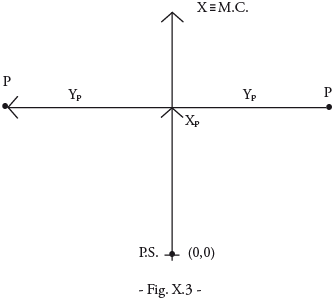
\includegraphics{repslatex-img81.png}
\end{marginfigure}
 

\ \ Por lo tanto los puntos situados sobre el meridiano central tienen
coordenadas:

\begin{equation*}
{l=0}
\end{equation*}
\begin{equation*}
{Y=0}
\end{equation*}
sobre el elipsoide y la carta, respectivamente.

\ \ La función (X.10) para dichos puntos se transforma en:

\begin{equation*}
{X=f\left(q\right)}
\end{equation*}
Los puntos del meridiano central están representados por puntos en una
recta, eje de las X, en tal forma que sus distancias relativas son
iguales en la proyección y en el elipsoide.

\ \ De lo anterior se deduce la naturaleza de la (X.11), que expresa el
arco de meridiano del polo sur al punto considerado, por la variable
{\textquotedblleft}q{\textquotedblright} la que en cualquier momento se
puede reemplazar por la variable  ${\varphi }$.

\ \ La función que expresa tal magnitud, como se determinó en VIII.5
es:

\begin{equation*}
{S=\overset{{\varphi }}{\underset{{-\pi /2}}{\int }}{M\cdot
\mathit{d\varphi }}}
\end{equation*}
De modo que se tiene:

\ \  ${S=f\left(q\right)}$  (X.12)

Para encontrar las coordenadas X e Y de puntos que no se encuentran
sobre el meridiano central, se desarrolla en serie de Taylor la
función de variable compleja (X.10) tomando como origen dicho
meridiano y como incremento la diferencia de longitud
{\textquotedblleft}l{\textquotedblright}.

Se obtiene por lo tanto: 

\begin{equation*}
{X+\normalsubformula{\text{iY}}=f\left(q\right)+\frac{\normalsubformula{\text{df}}\left(q\right)}{\normalsubformula{\text{dq}}}\cdot
\left(\normalsubformula{\text{il}}\right)+\frac{d^{{2}}f\left(q\right)}{\normalsubformula{\text{dq}}^{{2}}}\cdot
{\frac{\left(\normalsubformula{\text{il}}\right)^{{2}}}{2!}}+\frac{d^{{3}}f\left(q\right)}{\normalsubformula{\text{dq}}^{{3}}}\cdot
{\frac{\left(\normalsubformula{\text{il}}\right)}{3!}}^{{3}}+\text{.}\text{.}\text{.}}
\end{equation*}
O bien teniendo en cuenta la (X.12):

\begin{equation*}
{X+\normalsubformula{\text{iY}}=S+\frac{\normalsubformula{\text{dS}}}{\normalsubformula{\text{dq}}}\cdot
\left(\normalsubformula{\text{il}}\right)+\frac{d^{{2}}S}{\normalsubformula{\text{dq}}^{{2}}}\cdot
{\frac{\left(\normalsubformula{\text{il}}\right)^{{2}}}{2!}}+\frac{d^{{3}}S}{\normalsubformula{\text{dq}}^{{3}}}\cdot
{\frac{\left(\normalsubformula{\text{il}}\right)}{3!}}^{{3}}+\text{.}\text{.}\text{.}}
\end{equation*}
Los términos del desarrollo en serie pares son reales porque:

\begin{equation*}
{i^{{2}}=-1}
\end{equation*}
\begin{equation*}
{i^{{4}}=i^{{2}}\cdot i^{{2}}=\left(-1\right)\cdot \left(-1\right)=1}
\end{equation*}
\begin{equation*}
{i^{{6}}=i^{{4}}\cdot i^{{2}}=1\cdot \left(-1\right)=-1}
\end{equation*}
Por lo tanto los términos de derivadas pares corresponden a las X; los
términos de derivadas impares son imaginarios puros porque:

\begin{equation*}
{i^{{3}}=i^{{2}}\cdot i=-i}
\end{equation*}
\begin{equation*}
{i^{{5}}=i^{{3}}\cdot i^{{2}}=\left(-i\right)\cdot \left(-1\right)=i}
\end{equation*}
Por lo tanto corresponden a las Y. Es posible entonces separar las
variables reales e imaginarias:

\ \  ${X=S-\frac{d^{{2}}S}{\normalsubformula{\text{dq}}^{{2}}}\cdot
{\frac{l^{{2}}}{2}}+\frac{d^{{4}}S}{\normalsubformula{\text{dq}}^{{4}}}\cdot
{\frac{l}{\text{24}}}^{{4}}-\frac{d^{{6}}S}{\normalsubformula{\text{dq}}^{{6}}}\cdot
{\frac{l^{{6}}}{\text{720}}}+\text{.}\text{.}\text{.}}$  (X.13.a)


${Y=\frac{\normalsubformula{\text{dS}}}{\normalsubformula{\text{dq}}}\cdot
l-\frac{d^{{3}}S}{\normalsubformula{\text{dq}}^{{3}}}\cdot
{\frac{l}{6}}^{{3}}+\frac{d^{{5}}S}{\normalsubformula{\text{dq}}^{{5}}}\cdot
{\frac{l^{{5}}}{\text{120}}}-\text{.}\text{.}\text{.}}$  (X.13.b)

Se calculará el primer término de la serie:

\begin{equation*}
{\frac{\normalsubformula{\text{dS}}}{\normalsubformula{\text{dq}}}=\frac{\normalsubformula{\text{dS}}}{\mathit{d\varphi
}}\cdot {\frac{\mathit{d\varphi }}{\normalsubformula{\text{dq}}}}}
\end{equation*}
\begin{equation*}
{\normalsubformula{\text{dS}}=M\cdot \mathit{d\varphi }}
\end{equation*}
\begin{equation*}
{\frac{\normalsubformula{\text{dS}}}{\mathit{d\varphi }}=M}
\end{equation*}
\begin{equation*}
{\normalsubformula{\text{dq}}=\frac{M\cdot \mathit{d\varphi }}{N\cdot
\text{cos}\left(\varphi \right)}}
\end{equation*}
\begin{equation*}
{\frac{\mathit{d\varphi }}{\normalsubformula{\text{dq}}}=\frac{N\cdot
\text{cos}\left[\varphi \right]}{M}}
\end{equation*}
Por lo tanto:

[Warning: Draw object ignored][Warning: Draw object ignored]\ \ 
${\frac{\normalsubformula{\text{dS}}}{\normalsubformula{\text{dq}}}=M\cdot
{\frac{N\cdot \text{cos}\left(\varphi \right)}{M}}}$

\ \ 
${\frac{\normalsubformula{\text{dS}}}{\normalsubformula{\text{dq}}}=N\cdot
\text{cos}\left(\varphi \right)}$  (X.14)

\ \ Para hallar las sucesivas derivadas de
{\textquotedblleft}S{\textquotedblright} respecto de
{\textquotedblleft}q{\textquotedblright} se deriva como función de
función, primero respecto de la variable {\textquotedblleft}
${\varphi }${\textquotedblright} y luego por
{\textquotedblleft}q{\textquotedblright}. Llamando:

\begin{equation*}
{F^{{\normalsubformula{\text{II}}}}=\frac{d^{{2}}S}{\normalsubformula{\text{dq}}^{{2}}}=\frac{d}{\mathit{d\varphi
}}\left(\frac{\normalsubformula{\text{dS}}}{\normalsubformula{\text{dq}}}\right)\frac{\mathit{d\varphi
}}{\normalsubformula{\text{dq}}}}
\end{equation*}
\begin{equation*}
{\frac{d}{\mathit{d\varphi
}}\left(\frac{\normalsubformula{\text{dS}}}{\normalsubformula{\text{dq}}}\right)=\frac{d}{\mathit{d\varphi
}}\left[N\text{cos}\left(\varphi
\right)\right]=\frac{\normalsubformula{\text{dN}}}{\mathit{d\varphi
}}\cdot \text{cos}\left(\varphi \right)-N\cdot
\normalsubformula{\text{sen}}\left(\varphi \right)}
\end{equation*}
\begin{equation*}
{N=a\cdot \left[1-e^{{2}}\cdot
\normalsubformula{\text{sen}}^{{2}}\left(\varphi
\right)\right]^{{-1/2}}}
\end{equation*}
\begin{equation*}
{\frac{\normalsubformula{\text{dN}}}{\mathit{d\varphi }}=a\cdot
\left[1-e^{{2}}\cdot \normalsubformula{\text{sen}}^{{2}}\left(\varphi
\right)\right]^{{-3/2}}\cdot e^{{2}}\cdot
\normalsubformula{\text{sen}}\left(\varphi \right)\cdot
\text{cos}\left(\varphi \right)=\frac{N\cdot e^{{2}}\cdot
\normalsubformula{\text{sen}}\left(\varphi \right)\cdot
\text{cos}\left(\varphi \right)}{1-e^{{2}}\cdot
\normalsubformula{\text{sen}}^{{2}}\left(\varphi \right)}}
\end{equation*}
\begin{equation*}
{\frac{d}{\mathit{d\varphi
}}\left(\frac{\normalsubformula{\text{dS}}}{\normalsubformula{\text{dq}}}\right)=\left[\frac{N\cdot
e^{{2}}\cdot \normalsubformula{\text{sen}}\left(\varphi \right)\cdot
\text{cos}\left(\varphi \right)}{1-e^{{2}}\cdot
\normalsubformula{\text{sen}}^{{2}}\left(\varphi \right)}\right]\cdot
\text{cos}\left(\varphi \right)-N\cdot
\normalsubformula{\text{sen}}\left(\varphi \right)=}
\end{equation*}
\begin{equation*}
{=\frac{N\cdot e^{{2}}\cdot \normalsubformula{\text{sen}}\left(\varphi
\right)\cdot \text{cos}^{{2}}\left(\varphi \right)-N\cdot
\normalsubformula{\text{sen}}\left(\varphi \right)\cdot
\left[1-e^{{2}}\cdot \normalsubformula{\text{sen}}^{{2}}\left(\varphi
\right)\right]}{1-e^{{2}}\cdot
\normalsubformula{\text{sen}}^{{2}}\left(\varphi \right)}=}
\end{equation*}
 ${=\frac{\left[-N\cdot \normalsubformula{\text{sen}}\left(\varphi
\right)\right]\cdot \left[-e^{{2}}\cdot \text{cos}^{{2}}\left(\varphi
\right)+\left(1-e^{{2}}\cdot
\normalsubformula{\text{sen}}^{{2}}\left(\varphi
\right)\right)\right]}{1-e^{{2}}\cdot
\normalsubformula{\text{sen}}^{{2}}\left(\varphi
\right)}=\frac{\left[-N\cdot \normalsubformula{\text{sen}}\left(\varphi
\right)\right]\cdot \left(1-e^{{2}}\right)}{1-e^{{2}}\cdot
\normalsubformula{\text{sen}}^{{2}}\left(\varphi \right)}=}$

\begin{equation*}
{=\frac{\left(-a\right)\cdot \left(1-e^{{2}}\right)\cdot
\normalsubformula{\text{sen}}\left(\varphi
\right)}{\left[1-e^{{2}}\cdot
\normalsubformula{\text{sen}}^{{2}}\left(\varphi
\right)\right]^{{-3/2}}}}
\end{equation*}
\begin{equation*}
{\frac{d}{\mathit{d\varphi
}}\left(\frac{\normalsubformula{\text{dS}}}{\normalsubformula{\text{dq}}}\right)=-M\cdot
\normalsubformula{\text{sen}}\left(\varphi \right)}
\end{equation*}
Por lo tanto:

[Warning: Draw object ignored][Warning: Draw object ignored]\ \ 
${F^{{\normalsubformula{\text{II}}}}=-M\cdot
\normalsubformula{\text{sen}}\left(\varphi \right)\cdot {\frac{N\cdot
\text{cos}\left(\varphi \right)}{M}}}$

\ \  ${F^{{\normalsubformula{\text{II}}}}=\left(-N\right)\cdot
\normalsubformula{\text{sen}}\left(\varphi \right)\cdot
\text{cos}\left(\varphi \right)}$  (X.15)

En las deducciones de las derivadas restantes se usan las siguientes
abreviaturas auxiliares:

\begin{equation*}
{n^{{2}}=e'^{{2}}\cdot \text{cos}^{{2}}\left(\varphi \right)}
\end{equation*}
\begin{equation*}
{t=\normalsubformula{\text{tg}}\left(\varphi \right)}
\end{equation*}
\begin{equation*}
{e'^{{2}}=\frac{a^{{2}}-b^{{2}}}{a^{{2}}}}
\end{equation*}
Reemplazando estas abreviaturas en la segunda derivada:

\begin{equation*}
{F^{{\normalsubformula{\text{II}}}}=\left(-N\right)\cdot
\text{cos}\left(\varphi \right)\cdot
\normalsubformula{\text{sen}}\left(\varphi \right)\cdot
{\frac{\text{cos}\left(\varphi \right)}{\text{cos}\left(\varphi
\right)}}=\left(-N\right)\cdot \text{cos}^{{2}}\left(\varphi
\right)\cdot \normalsubformula{\text{tg}}\left(\varphi
\right)=\left(-N\right)\cdot \text{cos}^{{2}}\left(\varphi \right)\cdot
t}
\end{equation*}
La  ${\frac{\mathit{d\varphi }}{\normalsubformula{\text{dq}}}}$ se
expresa también en función de las nuevas abreviaturas introducidas,
de manera tal que:

\begin{equation*}
{\frac{\mathit{d\varphi
}}{\normalsubformula{\text{dq}}}=\frac{N}{M}\cdot
\text{cos}\left(\varphi \right)=\frac{a\cdot \left[1-e^{{2}}\cdot
\normalsubformula{\text{sen}}^{{2}}\left(\varphi
\right)\right]^{{3/2}}\cdot \text{cos}\left(\varphi
\right)}{\left[1-e^{{2}}\cdot
\normalsubformula{\text{sen}}^{{2}}\left(\varphi
\right)\right]^{{1/2}}\cdot a\cdot
\left(1-e^{{2}}\right)}=\frac{\left[1-e^{{2}}\cdot
\normalsubformula{\text{sen}}^{{2}}\left(\varphi
\right)\right]}{\left(1-e^{{2}}\right)}\cdot \text{cos}\left(\varphi
\right)}
\end{equation*}
Teniendo en cuenta que:

\begin{equation*}
{e'^{{2}}=\frac{e^{{2}}}{1-e^{{2}}}}
\end{equation*}
 ${\frac{\mathit{d\varphi
}}{\normalsubformula{\text{dq}}}=\left(\frac{1-e^{{2}}}{1-e^{{2}}}-\frac{e^{{2}}\cdot
\text{cos}^{{2}}\left(\varphi \right)}{1-e^{{2}}}\right)\cdot
\text{cos}\left(\varphi \right)=\left[1+e^{{2}}\cdot
\text{cos}^{{2}}\left(\varphi \right)\right]\cdot
\text{cos}\left(\varphi \right)}$

 ${\frac{\mathit{d\varphi
}}{\normalsubformula{\text{dq}}}=\left[1+n^{{2}}\right]\cdot
\text{cos}\left(\varphi \right)}$  (X.16)

Para hallar la tercera derivada se hace:

\begin{equation*}
{\frac{F^{{\normalsubformula{\text{II}}}}}{F^{{I}}}=\frac{\left(-N\right)\cdot
\text{cos}\left(\varphi \right)\cdot
\normalsubformula{\text{sen}}\left(\varphi \right)}{N\cdot
\text{cos}\left(\varphi
\right)}=-\normalsubformula{\text{sen}}\left(\varphi \right)}
\end{equation*}
Y se derivan ambos miembros respecto de
{\textquotedblleft}q{\textquotedblright}:

\begin{equation*}
{\frac{F^{{\normalsubformula{\text{III}}}}\cdot
F^{{I}}-F^{{\normalsubformula{\text{II}}}}\cdot
F^{{\normalsubformula{\text{II}}}}}{F^{{I}^{{2}}}}=\frac{F^{{\normalsubformula{\text{III}}}}}{F^{{I}}}-\frac{F^{{\normalsubformula{\text{II}}}^{{2}}}}{F^{{I}^{{2}}}}=-\text{cos}\left(\varphi
\right)\cdot {\frac{\mathit{d\varphi
}}{\normalsubformula{\text{dq}}}}=-\text{cos}^{{2}}\left(\varphi
\right)\cdot \left(1+n^{{2}}\right)}
\end{equation*}
\begin{equation*}
{F^{{\normalsubformula{\text{III}}}}=\left[-\text{cos}^{{2}}\left(\varphi
\right)\cdot
\left(1+n^{{2}}\right)+\frac{F^{{\normalsubformula{\text{II}}}^{{2}}}}{F^{{I}^{{2}}}}\right]\cdot
F^{{I}^{{2}}}}
\end{equation*}
[Warning: Draw object ignored][Warning: Draw object ignored]\ \ 
${F^{{\normalsubformula{\text{III}}}}=\left[-\text{cos}^{{2}}\left(\varphi
\right)\cdot \left(1+n^{{2}}\right)+\frac{N^{{2}}\cdot
\text{cos}^{{4}}\left(\varphi \right)\cdot t^{{2}}}{N^{{2}}\cdot
\text{cos}^{{2}}\left(\varphi \right)}\right]\cdot N\cdot
\text{cos}\left(\varphi \right)}$

\ \ 
${F^{{\normalsubformula{\text{III}}}}=\left[-\text{cos}^{{3}}\left(\varphi
\right)\right]\cdot \left(1-t^{{2}}+n^{{2}}\right)\cdot N}$  (X.17)

De manera similar se encuentran las siguientes derivadas:

\ \  ${F^{{\normalsubformula{\text{IV}}}}=\text{cos}^{{4}}\left(\varphi
\right)\cdot N\cdot t\cdot \left(5-t^{{2}}+9\cdot n^{{2}}+4\cdot
n^{{4}}\right)}$  (X.18)

 ${F^{{V}}=\text{cos}^{{5}}\left(\varphi \right)\cdot N\cdot
\left(5-\text{18}\cdot t^{{2}}+t^{{4}}+\text{14}\cdot
n^{{2}}-\text{58}\cdot t^{{2}}\cdot n^{{2}}+\text{13}\cdot
n^{{4}}-\text{64}\cdot t^{{2}}\cdot n^{{4}}+4\cdot
n^{{6}}-\text{24}\cdot t^{{2}}\cdot n^{{6}}\right)}$ (X.19)

\begin{equation*}
{F^{{\normalsubformula{\text{VI}}}}=\text{cos}^{{6}}\left(\varphi
\right)\cdot N\cdot t\cdot (\text{61}-\text{58}\cdot
t^{{2}}+t^{{4}}+\text{270}\cdot n^{{2}}-\text{330}\cdot t^{{2}}\cdot
n^{{2}}+\text{445}\cdot n^{{4}}-\text{680}\cdot t^{{2}}\cdot n^{{4}}+}
\end{equation*}
 ${+\text{44}\cdot n^{{6}}-\text{600}\cdot t^{{2}}\cdot
n^{{6}}+\text{88}\cdot n^{{8}}-\text{192}\cdot t^{{2}}\cdot n^{{8}})}$ 
(X.20)

Reemplazando las expresiones de las derivadas (X.14), (X.15), (X.17),
(X.18), (X.19) y (X.20) en los desarrollos en serie de (X.13.a) y
(X.13.b) dará las coordenadas de los puntos de la carta con las
abscisas contadas a partir del polo sur y las ordenadas a partir del
meridiano central de la faja.

\ \ Las coordenadas X e Y en la proyección Gauss- Kr\"uger resultan
entonces:

\begin{equation*}
{X=S+\frac{l^{{2}}\cdot \text{cos}^{{2}}\left(\varphi \right)\cdot
N\cdot t}{2}+\frac{l^{{4}}\cdot \text{cos}^{{4}}\left(\varphi
\right)\cdot N\cdot t}{\text{24}}\cdot \left(5-t^{{2}}+9\cdot
n^{{2}}+4\cdot n^{{4}}\right)+}
\end{equation*}
 ${+{\frac{l^{{6}}\cdot \text{cos}^{{6}}\left(\varphi \right)\cdot
N\cdot t}{\text{720}}}\cdot (\text{61}-\text{58}\cdot
t^{{2}}+t^{{4}}+\text{270}\cdot n^{{2}}-\text{330}\cdot t^{{2}}\cdot
n^{{2}}+\text{445}\cdot n^{{4}}-\text{680}\cdot t^{{2}}\cdot
n^{{4}}+}$\ \  ${+\text{44}\cdot n^{{6}}-\text{600}\cdot t^{{2}}\cdot
n^{{6}}+\text{88}\cdot n^{{8}}-\text{192}\cdot t^{{2}}\cdot n^{{8}})}$ 
(X.21.a)

\begin{equation*}
{Y=l\cdot \text{cos}\left(\varphi \right)\cdot N+\frac{l^{{3}}\cdot
\text{cos}^{{3}}\left(\varphi \right)\cdot N}{6}\cdot
\left(1-t^{{2}}+n^{{2}}\right)+\frac{l^{{5}}\cdot
\text{cos}^{{5}}\left(\varphi \right)\cdot N}{\text{120}}\cdot
(5-\text{18}\cdot t^{{2}}+t^{{4}}+}
\end{equation*}
 ${+\text{14}\cdot n^{{2}}-\text{58}\cdot t^{{2}}\cdot
n^{{2}}+\text{13}\cdot n^{{4}}-\text{64}\cdot t^{{2}}\cdot
n^{{4}}+4\cdot n^{{6}}-\text{24}\cdot t^{{2}}\cdot n^{{6}})}$  (X.21.b)

\ \ Estas últimas expresiones dan la representación conforme de una
parte de la superficie terrestre sobre un plano, o bien para toda la
extensión de la tierra. Se elige un meridiano central a partir del
cual se cuentan las cantidades
{\textquotedblleft}l{\textquotedblright}, positivas al Este y negativas
al Oeste.

\ \ Las fórmulas (X.21.a) y (X.21.b) dan va valores negativos de las Y
para los puntos situados al Oeste del meridiano central y habría que
hacer distinción de signos para las ordenadas.

\ \ El sistema de fajas meridianas introducidas por Kr\"uger están
limitadas en 3{\textordfeminine} de longitud,
1{\textordfeminine}30{\textquoteright} a cada lado del meridiano
central. Se debe distinguir por lo tanto las coordenadas de las
siguientes longitudes respecto de Greenwich: -72{\textordmasculine},
-69{\textordmasculine}, -66{\textordmasculine}, -63{\textordmasculine},
- 60{\textordmasculine}, -57{\textordmasculine},
-54{\textordmasculine}.

\ \ Con el fin de evitar coordenadas Y negativas, se ha convenido en
aumentar en 500.000 a todas las Y, de modo que resultan menores que
500.000 al Oeste del meridiano central, pero positivas y superiores a
500.000 al Este. Se elige este valor debido a que ninguna coordenada Y
lo supera dentro de una misma faja.

\ \ Como a un determinado par de coordenadas le debe corresponder un
solo punto dentro del sistema, lo cual con las convenciones adoptadas
hasta ahora no sería el caso, dado que en las siete fajas existen
siete puntos con las mismas coordenadas, se aumentan las ordenadas Y en
números enteros de millones según la faja de que se trata.

\ \ Así se atribuyen a los siete meridianos centrales los siguientes
números de faja, que corresponden al número entero de millones que
se antepone a las Y, resultando las siguientes coordenadas para dichos
meridianos:

\begin{center}
\tablehead{}
\begin{supertabular}{|m{2.848cm}|m{2.975cm}|m{4.263cm}|}
\hline
\centering Meridiano &
\centering N{\textordmasculine} de faja &
\centering\arraybslash Ordenada Y\\\hline
\centering {}-72{\textordmasculine} &
\centering 1 &
\centering\arraybslash 1.500.000\\\hline
\centering {}-69{\textordmasculine} &
\centering 2 &
\centering\arraybslash 2.500.000\\\hline
\centering {}-66{\textordmasculine} &
\centering 3 &
\centering\arraybslash 3.500.000\\\hline
\centering {}-63{\textordmasculine} &
\centering 4 &
\centering\arraybslash 4.500.000\\\hline
\centering {}-60{\textordmasculine} &
\centering 5 &
\centering\arraybslash 5.500.000\\\hline
\centering {}-57{\textordmasculine} &
\centering 6 &
\centering\arraybslash 6.500.000\\\hline
\centering {}-54{\textordmasculine} &
\centering 7 &
\centering\arraybslash 7.500.000\\\hline
\end{supertabular}
\end{center}
\ \ Llamando Y{\textquoteright} al valor obtenido de la expresión
(X.21.b) con las modificaciones descriptas, el valor de la coordenada Y
en el sistema Gauss- Kr\"uger aplicado a la Argentina se transforma en:

\begin{equation*}
{Y=n\cdot t^{{6}}+\text{500}\text{.}\text{000}+Y'}
\end{equation*}
donde {\textquotedblleft}n{\textquotedblright} es el número de faja.

\ \ Las expresiones (X.21) corresponden al orden de precisión de los
trabajos fundamentales; en trabajos de menor precisión se podrá
prescindir de los términos {\textquotedblleft}t{\textquotedblright} y
{\textquotedblleft}n{\textquotedblright} con potencias superiores a 2.

\ \ Conocidas las coordenadas geográficas de los puntos, se calculan
las coordenadas Gauss- Kr\"uger de los mismos dentro de la faja que
corresponda.

\ \ Por razones prácticas, se extienden las coordenadas hasta
2{\textordmasculine} a cada lado del meridiano central. De esa manera
los puntos situados cerca de los bordes de faja tienen coordenadas en
los dos sistemas vecinos.

\ \ De esta manera cuando se realiza algún levantamiento que se
extiende en una faja vecina no necesita hacer uso de coordenadas en dos
sistemas distintos.

\ \ En las cartas topográficas se ha trazado una cuadrícula de
coordenadas Gauss- Kr\"uger en el borde de cada hoja. Frente a las
líneas del cuadriculado se han impreso las coordenadas en
kilómetros permitiendo determinar las coordenadas de cualquier punto
que interese.

\ \ Se deberá medir la distancia en X e Y que separa al punto
considerado de un cruce de cuadrícula próximo, tendiendo en cuenta
la escala de la carta, y se agregan esos valores a las coordenadas de
cruce elegido. Para la determinación de dichas distancias figuran en
la información marginal de la carta una escala de coordenadas.

\ \ La operación recíproca, es decir dado un par de coordenadas
ubicar dicho punto en la carta, también es posible por medio de la
cuadrícula. 

X.3.- TRANSFORMACIÓN DE COORDENADAS PLANAS EN GEOGRÁFICAS.

\ \ Se debe resolver el problema inverso del que se vio en el punto
anterior, planteando en forma general las siguientes ecuaciones:


${q+\normalsubformula{\text{il}}=F\left(x+\normalsubformula{\text{iy}}\right)}$
 (X.22)

Análogamente, se desarrollan en serie de Taylor:

\begin{equation*}
{q+\normalsubformula{\text{il}}=F\left(x\right)+F^{{I}}\left(x\right)\left(\normalsubformula{\text{iy}}\right)-F^{{\normalsubformula{\text{II}}}}\left(x\right)\frac{y^{{2}}}{2}+F^{{\normalsubformula{\text{III}}}}\left(x\right)\frac{\left(\normalsubformula{\text{iy}}\right)^{{3}}}{3!}+F^{{\normalsubformula{\text{IV}}}}\left(x\right)\frac{y^{{4}}}{4!}}
\end{equation*}
Separando la parte real y la imaginaria:

\begin{equation*}
{q=F\left(x\right)-F^{{\normalsubformula{\text{II}}}}\left(x\right)\frac{y^{{2}}}{2}+F^{{\normalsubformula{\text{IV}}}}\left(x\right)\frac{y^{{2}}}{\text{24}}-\text{.}\text{.}\text{.}}
\end{equation*}
 (X.23)

\begin{equation*}
{l=F^{{I}}\left(x\right)y-F^{{\normalsubformula{\text{III}}}}\left(x\right)\frac{y^{{3}}}{6}+F^{{V}}\left(x\right)\frac{y^{{5}}}{\text{120}}-\text{.}\text{.}\text{.}}
\end{equation*}
Estas últimas expresiones resultan de la condición de conformidad de
la transformación de un plano al elipsoide. De la misma forma que se
realizó en la proyección Gauss- Kr\"uger, se introducen ciertas
condiciones para la transformación.

\begin{marginfigure}
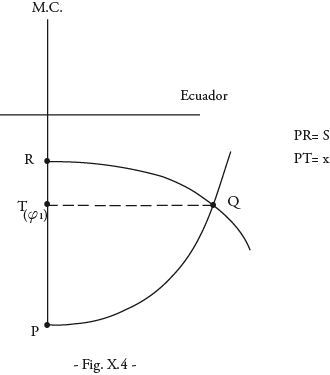
\includegraphics{repslatex-img82.png}
\end{marginfigure}
 

Para y=0 debe ser l=0; por lo tanto:

 ${F\left(x\right)=q_{{1}}}$  (X.24)

En la figura (X.4), S es el arco de meridiano del polo sur hasta la
latitud del punto Q; X es la coordenada Gauss, distancia del polo sur
al pie de la perpendicular desde Q al meridiano central, que se
denomina T; a la latitud del punto T se la denomina  ${\varphi
_{{1}}}$. Por lo tanto  ${q_{{1}}}$ se calcula en función de 
${\varphi _{{1}}}$.

Este valor puede ser obtenido en función de la coordenada X, en efecto
de la (VIII.13), arco de meridiano del polo sur a una altitud
cualquiera.

 ${X=S=\alpha \cdot \varphi _{{1}}+\alpha \cdot {\frac{\pi }{2}}+\beta
\cdot \normalsubformula{\text{sen}}\left(2\cdot \varphi
_{{1}}\right)+\gamma \cdot \normalsubformula{\text{sen}}\left(4\cdot
\varphi _{{1}}\right)+\delta \cdot
\normalsubformula{\text{sen}}\left(6\cdot \varphi
_{{1}}\right)+\varepsilon \cdot
\normalsubformula{\text{sen}}\left(8\cdot \varphi
_{{1}}\right)+\text{.}\text{.}\text{.}}$ (VIII.13)

El valor de  ${\varphi _{{1}}}$ se obtiene por aproximaciones sucesivas:

\begin{equation*}
{X=\alpha \cdot \left(\varphi _{{1,1}}+\frac{\pi }{2}\right)}
\end{equation*}
\begin{equation*}
{\varphi _{{1,1}}=\frac{X}{\alpha }-\frac{\pi }{2}}
\end{equation*}
Luego se introduce este primer valor de la latitud en la (VIII.13) para
obtener una segunda aproximación del valor de la latitud.

\begin{equation*}
{\varphi _{{1,2}}=\frac{1}{\alpha }\left(x-\alpha \cdot {\frac{\pi
}{2}}-\beta \cdot \normalsubformula{\text{sen}}\left(2\cdot \varphi
_{{1,1}}\right)-\gamma \cdot \normalsubformula{\text{sen}}\left(4\cdot
\varphi _{{1,1}}\right)-\delta \cdot
\normalsubformula{\text{sen}}\left(6\cdot \varphi
_{{1,1}}\right)-\varepsilon \cdot
\normalsubformula{\text{sen}}\left(8\cdot \varphi
_{{1,1}}\right)\right)}
\end{equation*}
\begin{equation*}
{\varphi _{{1,2}}=\left(\frac{x}{\alpha }-\frac{\pi
}{2}\right)-\frac{\beta }{\alpha }\cdot
\normalsubformula{\text{sen}}\left(2\cdot \varphi
_{{1,1}}\right)-\frac{\gamma }{\alpha }\cdot
\normalsubformula{\text{sen}}\left(4\cdot \varphi
_{{,\text{11}}}\right)-\frac{\delta }{\alpha }\cdot
\normalsubformula{\text{sen}}\left(6\cdot \varphi
_{{1,1}}\right)-\frac{\varepsilon }{\alpha }\cdot
\normalsubformula{\text{sen}}\left(8\cdot \varphi _{{1,1}}\right)}
\end{equation*}
\begin{equation*}
{\varphi _{{1,2}}=\varphi _{{1,1}}-\frac{1}{\alpha }\left[\beta \cdot
\normalsubformula{\text{sen}}\left(2\cdot \varphi
_{{1,1}}\right)-\gamma \cdot \normalsubformula{\text{sen}}\left(4\cdot
\varphi _{{1,1}}\right)-\delta \cdot
\normalsubformula{\text{sen}}\left(6\cdot \varphi
_{{1,1}}\right)-\varepsilon \cdot
\normalsubformula{\text{sen}}\left(8\cdot \varphi
_{{1,1}}\right)\right]}
\end{equation*}

\begin{equation*}
{\varphi _{{1,3}}=\varphi _{{1,1}}-\left[\beta \cdot
\normalsubformula{\text{sen}}\left(2\cdot \varphi
_{{1,2}}\right)+\gamma \cdot \normalsubformula{\text{sen}}\left(4\cdot
\varphi _{{1,2}}\right)+\delta \cdot
\normalsubformula{\text{sen}}\left(6\cdot \varphi
_{{1,2}}\right)+\varepsilon \cdot
\normalsubformula{\text{sen}}\left(8\cdot \varphi
_{{1,2}}\right)\right]}
\end{equation*}
Se sigue iterando hasta que en la (VIII.13) introduciendo  ${\varphi
_{{1,j}}}$ dé como resultado el valor de X ingresado.

Para resolver las (X.23) se debe recordar:

\begin{equation*}
{\normalsubformula{\text{dq}}=\frac{M\cdot \mathit{d\varphi }}{N\cdot
\text{cos}\left(\varphi \right)}}
\end{equation*}
Donde:

\begin{equation*}
{q=\int {\frac{M\cdot \mathit{d\varphi }}{N\cdot \text{cos}\left(\varphi
\right)}}}
\end{equation*}
Por lo tanto:

\begin{equation*}
{\varphi =f\left(q\right)=f\left[q_{{1}}+\left(q-q_{{1}}\right)\right]}
\end{equation*}
Desarrollando en serie, tomando a  ${\left(q-q_{{1}}\right)}$ como
incremento, se tiene:

\ \  ${\varphi =\varphi _{{1}}+\frac{\mathit{d\varphi
}}{\normalsubformula{\text{dq}}}\left(q-q_{{1}}\right)+\frac{d^{{2}}\varphi
}{\normalsubformula{\text{dq}}^{{2}}}\left(q-q_{{1}}\right)^{{2}}+\text{.}\text{.}\text{.}}$

Y por la (X.23) y (X.24) se tiene que:

\begin{equation*}
{\varphi =\varphi
_{{1}}-\left[F^{{\normalsubformula{\text{II}}}}\left(x\right)\frac{y^{{2}}}{2}-F^{{\normalsubformula{\text{IV}}}}\left(x\right)\frac{y^{{4}}}{\text{24}}\right]\cdot
{\frac{\mathit{d\varphi }}{\normalsubformula{\text{dq}}}}}
\end{equation*}
Para encontrar las expresiones se hallan las derivadas:

\begin{equation*}
{F^{{I}}\left(x\right)=\frac{\normalsubformula{\text{dq}}}{\normalsubformula{\text{dx}}}=\frac{\normalsubformula{\text{dq}}}{\mathit{d\varphi
}}\cdot {\frac{\mathit{d\varphi }}{\normalsubformula{\text{dx}}}}}
\end{equation*}
\ \  ${\frac{\normalsubformula{\text{dq}}}{\mathit{d\varphi
}}=\frac{M}{N\cdot \text{cos}\left(\varphi \right)}}$  ;  
${\frac{\mathit{d\varphi }}{\normalsubformula{\text{dx}}}=\frac{1}{M}}$

\begin{equation*}
{\frac{\mathit{d\varphi
}}{\normalsubformula{\text{dx}}}=\frac{1}{\text{cos}\left(\varphi
\right)}}
\end{equation*}
La segunda derivada se obtiene haciendo:

\begin{equation*}
{\frac{d^{{2}}q}{\normalsubformula{\text{dx}}^{{2}}}=\frac{d}{\mathit{d\varphi
}}\left(\frac{\normalsubformula{\text{dq}}}{\normalsubformula{\text{dx}}}\right)\frac{\mathit{d\varphi
}}{\normalsubformula{\text{dx}}}}
\end{equation*}
\ \ Omitiendo el cálculo de ésta y las derivadas de orden superior,
como así también ciertas transformaciones, se obtienen las
siguientes expresiones:

\begin{equation*}
{l=\frac{y}{N_{{1}}\cdot \text{cos}\left(\varphi _{{1}}\right)}\cdot
\left[1-\frac{y^{{2}}}{6\cdot N_{{1}}^{{2}}}\cdot \left(1+2\cdot
t_{{1}}^{{2}}+n_{{1}}^{{2}}\right)+\frac{y^{{4}}}{\text{120}\cdot
N_{{1}}^{{4}}}\cdot \left(5+\text{28}\cdot t_{{1}}^{{2}}+\text{24}\cdot
t_{{1}}^{{4}}+6\cdot n_{{1}}^{{2}}+8\cdot n_{{1}}^{{2}}\cdot
t_{{1}}^{{2}}\right)\right]}
\end{equation*}
(X.25.a)

 ${\varphi =\varphi _{{1}}-\frac{y^{{2}}}{2\cdot N_{{1}}\cdot
M_{{1}}}\cdot t_{{1}}\cdot \left[1-\frac{y^{{2}}}{\text{12}\cdot
N_{{1}}^{{2}}}\cdot \left(5+3\cdot t_{{1}}^{{2}}+n_{{1}}^{{2}}-9\cdot
t_{{1}}^{{2}}\cdot n_{{1}}^{{2}}\right)+\frac{y^{{4}}}{\text{360}\cdot
N_{{1}}^{{4}}}\cdot \left(\text{61}+\text{90}\cdot
t_{{1}}^{{2}}+\text{45}\cdot t_{{1}}^{{4}}\right)\right]}$(X.25.b)

Expresiones en las que el resultado se obtiene en radianes.

X.4.- CONVERGENCIA DE MERIDIANOS.

\begin{marginfigure}
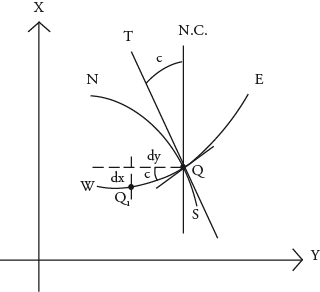
\includegraphics{repslatex-img83.png}
\end{marginfigure}
 

\ \ Considerando la figura (X.5), NS representa la imagen del meridiano
que pasa por Q, WE el paralelo que pasa por el mismo punto, NC la
dirección paralela al meridiano central, es decir el norte de
cuadrícula.

\ \ El ángulo {\textquotedblleft}c{\textquotedblright} formado por la
tangente a NS en Q y la dirección NC, se denomina convergencia de
meridianos plana.

\ \ Considerando un punto Q1 infinitamente próximo, la diferencia de
coordenadas entre éste y Q es dx y dy. Del triángulo elemental de
la figura:


${\normalsubformula{\text{tg}}\left(c\right)=\frac{\normalsubformula{\text{dx}}}{\normalsubformula{\text{dy}}}}$
 (X.26)

 ${\frac{\normalsubformula{\text{dx}}}{\normalsubformula{\text{dy}}}}$
se halla de la ecuación de la curva WE, en la cual la latitud es
constante por tratarse de un paralelo y la (X.26) puede escribirse:

\begin{equation*}
{\normalsubformula{\text{tg}}\left(c\right)=\frac{\normalsubformula{\text{dx}}/\normalsubformula{\text{dl}}}{\normalsubformula{\text{dy}}/\normalsubformula{\text{dl}}}}
\end{equation*}
Las derivadas 
${\frac{\normalsubformula{\text{dx}}}{\normalsubformula{\text{dl}}}}$ y
 ${\frac{\normalsubformula{\text{dy}}}{\normalsubformula{\text{dl}}}}$
se obtienen de diferenciar las expresiones de las coordenadas Gauss
(X.21.a) y (X.21.b), obteniéndose como primera aproximación:

\begin{equation*}
{\frac{\normalsubformula{\text{dx}}}{\normalsubformula{\text{dy}}}=l\cdot
\text{cos}^{{2}}\left(\varphi \right)\cdot N\cdot t}
\end{equation*}
\begin{equation*}
{\frac{\normalsubformula{\text{dy}}}{\normalsubformula{\text{dl}}}=N\cdot
\text{cos}\left(\varphi \right)}
\end{equation*}
La convergencia de meridianos, también como primera aproximación,
será:

\begin{equation*}
{\normalsubformula{\text{tg}}\left(c\right)=\frac{\normalsubformula{\text{dx}}/\normalsubformula{\text{dl}}}{\normalsubformula{\text{dy}}/\normalsubformula{\text{dl}}}=\frac{l\cdot
\text{cos}^{{2}}\left(\varphi \right)\cdot N\cdot t}{N\cdot
\text{cos}\left(\varphi \right)}=l\cdot
\normalsubformula{\text{sen}}\left(\varphi \right)}
\end{equation*}
\ \  ${\normalsubformula{\text{tg}}\left(c\right)=l\cdot
\normalsubformula{\text{sen}}\left(\varphi \right)}$  (X.27)

Con {\textquotedblleft}l{\textquotedblright} en radianes.

\ \ Como resultado de la diferenciación de las expresiones de las
coordenadas Gauss con respecto a
{\textquotedblleft}l{\textquotedblright}, considerando todos los
miembros y la (X.27), se obtiene:

\begin{equation*}
{\normalsubformula{\text{tg}}\left(c\right)=l\cdot
\normalsubformula{\text{sen}}\left(\varphi
\right)-\frac{l^{{3}}}{3}\cdot
\normalsubformula{\text{sen}}\left(\varphi \right)\cdot
\text{cos}^{{2}}\left(\varphi \right)\cdot \left(1+t^{{2}}+3\cdot
n^{{2}}+2n^{{4}}\right)+\frac{l^{{5}}}{\text{15}}\cdot
\normalsubformula{\text{sen}}\left(\varphi \right)\cdot
\text{cos}^{{4}}\left(\varphi \right)\cdot \left(2+4\cdot t+2\cdot
t^{{4}}\right)}
\end{equation*}
Como

\begin{equation*}
{c=\normalsubformula{\text{tg}}\left(c\right)-\frac{l^{{3}}}{3}\cdot
\normalsubformula{\text{tg}}^{{3}}\left(c\right)-\frac{l^{{5}}}{5}\cdot
\normalsubformula{\text{tg}}^{{5}}\left(c\right)}
\end{equation*}
 ${c=l\cdot \normalsubformula{\text{sen}}\left(\varphi
\right)+\frac{l^{{3}}}{3}\cdot
\normalsubformula{\text{sen}}\left(\varphi \right)\cdot
\text{cos}^{{2}}\left(\varphi \right)\cdot \left(1+3\cdot
n^{{2}}+2n^{{4}}\right)+\frac{l^{{5}}}{\text{15}}\cdot
\normalsubformula{\text{sen}}\left(\varphi \right)\cdot
\text{cos}^{{4}}\left(\varphi \right)\cdot \left(2-t^{{2}}\right)}$ 
(X.28.a)

Si se desea la convergencia en función de las coordenadas planas, se
obtiene reemplazando {\textquotedblleft}l{\textquotedblright} por las
coordenadas rectangulares

 ${d=\frac{y}{N_{{1}}}\cdot t_{{1}}\cdot \left[1-\frac{y^{{2}}}{3\cdot
N_{{1}}^{{2}}}\cdot \left(1+t_{{1}}^{{2}}-n_{{1}}^{{2}}-2\cdot
n_{{1}}^{{4}}\right)+\frac{y^{{4}}}{N_{{1}}^{{4}}}\cdot
{\frac{\left(2+5\cdot t_{{1}}^{{2}}+3\cdot
t_{{1}}^{{4}}\right)}{\text{15}}}\right]}$  (X.28.b)

X.5.- MÓDULO DE DEFORMACIÓN.

\ \ Por tratarse de una proyección conforme, el módulo de
deformación lineal o factor de escala varía de acuerdo a las
coordenadas pero una vez fijadas, el módulo es el mismo en cualquier
dirección.

\ \ De la (IX.2)

\begin{equation*}
{m^{{2}}=\frac{\normalsubformula{\text{ds}}^{{2}}}{\normalsubformula{\text{dS}}^{{2}}}=\frac{\left(\normalsubformula{\text{dx}}\right)^{{2}}+\left(\normalsubformula{\text{dy}}\right)^{{2}}}{\left(M\cdot
\mathit{d\varphi }\right)^{{2}}+\left(N\cdot \text{cos}\left(\varphi
\right)\cdot \normalsubformula{\text{dl}}\right)^{{2}}}}
\end{equation*}
\ \ 
${m^{{2}}=\frac{\left(\normalsubformula{\text{dy}}\right)^{{2}}\cdot
\left[1+\left(\normalsubformula{\text{dx}}/\normalsubformula{\text{dy}}\right)^{{2}}\right]}{\left(\normalsubformula{\text{dl}}\right)^{{2}}\cdot
N^{{2}}\cdot \text{cos}^{{2}}\left(\varphi \right)\cdot
\left[1+\left(\frac{M\cdot \mathit{d\varphi }}{N\cdot
\text{cos}\left(\varphi \right)\cdot
\normalsubformula{\text{dl}}}\right)^{{2}}\right]}}$

\begin{equation*}
{m^{{2}}=\left(\frac{\normalsubformula{\text{dy}}}{\normalsubformula{\text{dl}}}\right)^{{2}}\cdot
{\frac{1+\left(\normalsubformula{\text{dx}}/\normalsubformula{\text{dy}}\right)^{{2}}}{N^{{2}}\cdot
\text{cos}^{{2}}\left(\varphi \right)\cdot \left[1+\left(\frac{M\cdot
\mathit{d\varphi }}{N\cdot \text{cos}\left(\varphi \right)\cdot
\normalsubformula{\text{dl}}}\right)^{{2}}\right]}}}
\end{equation*}
Donde

\begin{equation*}
{1+\left(\normalsubformula{\text{dx}}/\normalsubformula{\text{dy}}\right)^{{2}}=1+\normalsubformula{\text{tg}}^{{2}}\left(c\right)=\text{sec}\left(c\right)}
\end{equation*}
Para el paralelo  ${\mathit{d\varphi }/\normalsubformula{\text{dl}}=0}$

\begin{equation*}
{m=\frac{\normalsubformula{\text{dy}}}{\normalsubformula{\text{dl}}}\cdot
{\frac{1}{N\cdot \text{cos}\left(\varphi \right)}}\cdot
\text{sec}\left(c\right)}
\end{equation*}
Calculando la derivada de {\textquotedblleft}y{\textquotedblright}
respecto de {\textquotedblleft}l{\textquotedblright} de la (X.21.b),
sustituyendo el valor de {\textquotedblleft}c{\textquotedblright}, se
obtiene:

 ${m=1+l^{{2}}\cdot \text{cos}^{{2}}\left(\varphi \right)\cdot
\left(1+n^{{2}}\right)+\frac{l^{{4}}\cdot \text{cos}^{{4}}\left(\varphi
\right)}{\text{24}}\cdot \left(5-t^{{2}}+\text{14}\cdot
n^{{2}}-\text{28}\cdot t^{{2}}\cdot n^{{2}}\right)}$  (X.29.a)

Expresión en la cual {\textquotedblleft}l{\textquotedblright} se
introduce en radianes.

\ \ Si se desea conocer la deformación lineal en función de las
coordenadas planas, se deduce:

\ \  ${m=1+\frac{y^{{2}}}{2\cdot R^{{2}}}+\frac{y^{{4}}}{\text{24}\cdot
R^{{4}}}}$  (X.29.b)

Donde:

\begin{equation*}
{R=\sqrt{M_{{1}}\cdot N_{{1}}}}
\end{equation*}
X.6.- DEFORMACIONES LINEALES.

\ \ Cuando se desea conocer la deformación de una distancia finita,
tendiendo en cuenta que:

\begin{equation*}
{m=\frac{\normalsubformula{\text{dl}}}{\normalsubformula{\text{dL}}}}
\end{equation*}
\begin{equation*}
{L=\overset{{l}}{\underset{{o}}{\int
}}{\frac{\normalsubformula{\text{dl}}}{m}}}
\end{equation*}
O bien:

\begin{equation*}
{l=\overset{{L}}{\underset{{o}}{\int }}{m\cdot
\normalsubformula{\text{dL}}}}
\end{equation*}
Donde {\textquotedblleft}L{\textquotedblright} es la distancia sobre el
elipsoide, {\textquotedblleft}l{\textquotedblright} es la
correspondiente en el plano y {\textquotedblleft}m{\textquotedblright}
es el módulo de deformación lineal, por lo tanto:

\begin{equation*}
{L=\overset{{l}}{\underset{{o}}{\int }}{\left(1+\frac{y^{{2}}}{2\cdot
R^{{2}}}+\frac{y^{{4}}}{\text{24}\cdot
R^{{2}}}\right)}^{{-1}}\normalsubformula{\text{dl}}}
\end{equation*}
Se desprecia el término de cuarto orden lo cual es aceptable hasta
unos 3 grados del meridiano central.

\begin{equation*}
{L=\overset{{l}}{\underset{{o}}{\int }}{\left(1+\frac{y^{{2}}}{2\cdot
R^{{2}}}\right)}^{{-1}}\normalsubformula{\text{dl}}}
\end{equation*}
O bien desarrollando el binomio:

\begin{equation*}
{L=\overset{{l}}{\underset{{o}}{\int }}{\left(1-\frac{y^{{2}}}{2\cdot
R^{{2}}}\right)}\normalsubformula{\text{dl}}}
\end{equation*}

\begin{marginfigure}
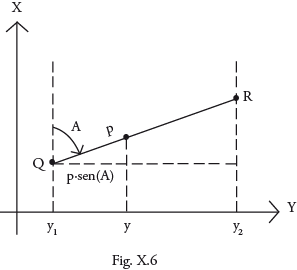
\includegraphics{repslatex-img84.png}
\end{marginfigure}
 

Sea {\textquotedblleft}p{\textquotedblright} en la figura (X.6) la
distancia del elemento {\textquotedblleft}dl{\textquotedblright} a
partir de {\textquotedblleft}Q{\textquotedblright}, designando
{\textquotedblleft}y1{\textquotedblright} ordenada del punto Q y  por
{\textquotedblleft}A{\textquotedblright} ángulo de dirección o
acimut de cuadrícula, se tiene que:

\begin{equation*}
{y=y_{{1}}+p\cdot \normalsubformula{\text{sen}}\left(A\right)}
\end{equation*}
Por lo tanto:

\ \  ${L=\overset{{p=l}}{\underset{{p=o}}{\int
}}{\left(1-\frac{\left(y_{{1}}+p\cdot
\normalsubformula{\text{sen}}\left(A\right)\right)^{{2}}}{2\cdot
R^{{2}}}\right)}\normalsubformula{\text{dp}}}$

\begin{equation*}
{L=\overset{{p=l}}{\underset{{p=o}}{\int
}}{\left(1-\frac{y_{{1}}^{{2}}+2\cdot y_{{1}}p\cdot
\normalsubformula{\text{sen}}\left(A\right)+p^{{2}}\cdot
\normalsubformula{\text{sen}}^{{2}}\left(A\right)}{2\cdot
R^{{2}}}\right)}\normalsubformula{\text{dp}}}
\end{equation*}
[Warning: Draw object ignored]

[Warning: Draw object ignored]\ \  ${L=p-\frac{y_{{1}}^{{2}}\cdot
p}{2\cdot R^{{2}}}-\frac{2\cdot y_{{1}}\cdot p^{{2}}\cdot
\normalsubformula{\text{sen}}\left(A\right)}{2\cdot 2\cdot
R^{{2}}}-\frac{p^{{3}}\cdot
\normalsubformula{\text{sen}}^{{2}}\left(A\right)}{6\cdot
R^{{2}}}|_{{0}}^{{l}}}$

\begin{equation*}
{L=p\cdot \left[1-\frac{y_{{1}}^{{2}}}{2\cdot
R^{{2}}}-\frac{y_{{1}}\cdot p\cdot
\normalsubformula{\text{sen}}\left(A\right)}{2\cdot
R^{{2}}}-\frac{p^{{2}}\cdot
\normalsubformula{\text{sen}}^{{2}}\left(A\right)}{6\cdot
R^{{2}}}\right]|_{{0}}^{{l}}}
\end{equation*}
\begin{equation*}
{L=l\cdot \left[1-\frac{y_{{1}}^{{2}}}{2\cdot
R^{{2}}}-\frac{y_{{1}}\cdot l\cdot
\normalsubformula{\text{sen}}\left(A\right)}{2\cdot
R^{{2}}}-\frac{l^{{2}}\cdot
\normalsubformula{\text{sen}}^{{2}}\left(A\right)}{6\cdot
R^{{2}}}\right]}
\end{equation*}
Teniendo en cuenta que

\begin{equation*}
{\mathit{\Delta y}=y_{{2}}-y_{{1}}}
\end{equation*}
\begin{equation*}
{\mathit{\Delta y}=l\cdot \normalsubformula{\text{sen}}\left(A\right)}
\end{equation*}
\begin{equation*}
{L=l\cdot \left[1-\frac{y_{{1}}^{{2}}}{2\cdot
R^{{2}}}-\frac{y_{{1}}\cdot \left(y_{{2}}-y_{{1}}\right)}{2\cdot
R^{{2}}}-\frac{\left(y_{{2}}-y_{{1}}\right)^{{2}}}{6\cdot
R^{{2}}}\right]}
\end{equation*}
Multiplicando y elevando al cuadrado el paréntesis y operando se
llega:

\begin{equation*}
{L=l\cdot \left[1-\frac{\left(y_{{1}}^{{2}}+y_{{1}}\cdot
y_{{2}}+y_{{2}}^{{2}}\right)}{6\cdot R^{{2}}}\right]}
\end{equation*}
El módulo de deformación de una distancia finita será:

\begin{equation*}
{\frac{l}{L}=\left[1-\frac{\left(y_{{1}}^{{2}}+y_{{1}}\cdot
y_{{2}}+y_{{2}}^{{2}}\right)}{6\cdot R^{{2}}}\right]^{{-1}}}
\end{equation*}
O bien

\ \  ${\frac{l}{L}=1+\frac{\left(y_{{1}}^{{2}}+y_{{1}}\cdot
y_{{2}}+y_{{2}}^{{2}}\right)}{6\cdot R^{{2}}}}$  (X.30.a)

Donde:

 ${R=\sqrt{M_{{1}}\cdot N_{{1}}}}$  ;   ${\varphi =\frac{\varphi
_{{2}}+\varphi _{{1}}}{2}}$

En algunos casos es suficiente con tomar un valor promedio de la
coordenada {\textquotedblleft}y{\textquotedblright}, entonces:

\begin{equation*}
{y_{{m}}=\frac{y_{{2}}+y_{{1}}}{2}}
\end{equation*}
Reemplazando en (X.30.a)

\ \  ${\frac{l}{L}=1+\frac{y_{{m}}^{{2}}}{2\cdot R^{{2}}}}$  (X.30.b)

X.7.- CORRECCIÓN ANGULAR.

\ \ En las proyecciones conformes los ángulos y las direcciones se
trasladan al elipsoide sin deformación pero la línea geodésica no
queda representada por una recta sino por alguna curva.

\begin{marginfigure}
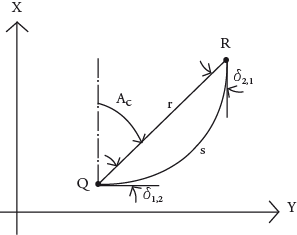
\includegraphics{repslatex-img85.png}
\end{marginfigure}
 

\ \ La conformidad se cumple en las tangentes a la curva que representa
a la línea geodésica. Si se mide un acimut en la carta respecto de
la línea recta que une los puntos del plano, se debe introducir una
corrección conocida como corrección del arco a la cuerda o
corrección por curvatura de la representación de la línea
geodésica sobre un plano.

\ \ Se llega a la siguiente expresión suficientemente aproximada para
cualquier aplicación práctica:

\ \  ${\delta _{{1,2}}=\frac{\left(x_{{2}}-x_{{1}}\right)\cdot
\left(2\cdot y_{{1}}+y_{{2}}\right)}{6\cdot M\cdot N}}$  (X.31.a)

\ \  ${\delta _{{2,1}}=\frac{\left(x_{{1}}-x_{{2}}\right)\cdot
\left(2\cdot y_{{2}}+y_{{1}}\right)}{6\cdot M\cdot N}}$

El resultado de la corrección viene expresado en radianes.

Tomando un valor promedio de la coordenada
{\textquotedblleft}y{\textquotedblright}, se tiene:

\begin{equation*}
{\delta _{{1,2}}=\frac{\left(x_{{2}}-x_{{1}}\right)\cdot \left(3\cdot
y_{{m}}\right)}{6\cdot M\cdot N}}
\end{equation*}
\ \  ${\delta _{{1,2}}=\frac{\mathit{\Delta x}\cdot y_{{m}}}{3\cdot
M\cdot N}}$  (X.41.b)

Donde es inmediato que:

\begin{equation*}
{\delta _{{1,2}}=-\delta _{{2,1}}}
\end{equation*}
\ \ La distancia de la línea recta que une los puntos debe ser
corregida llamando a ésta {\textquotedblleft}r{\textquotedblright} y
a la imagen de la línea geodésica
{\textquotedblleft}s{\textquotedblright} se tiene que:

\ \  ${\normalsubformula{\text{dr}}=\normalsubformula{\text{ds}}\cdot
\text{cos}\left(\delta \right)}$  
${r=\overset{{s}}{\underset{{0}}{\int
}}{\normalsubformula{\text{ds}}\cdot \text{cos}\left(\delta \right)}}$

\ \  ${\normalsubformula{\text{dr}}=\normalsubformula{\text{ds}}\cdot
\left(1-\frac{\delta ^{{2}}}{2}\right)}$  
${\normalsubformula{\text{dr}}-\normalsubformula{\text{ds}}=-\left(\frac{\delta
^{{2}}}{2}\right)\cdot \normalsubformula{\text{ds}}}$

La diferencia entre {\textquotedblleft}r{\textquotedblright} y
{\textquotedblleft}s{\textquotedblright} es despreciable.

XI.1.- PROYECCIÓN TRANSVERSA DE MERCATOR. SISTEMA U.T.M.

\ \ El sistema U.T.M. (Universal Transverse Mercator) de la proyección
de Gauss fue recomendado por la Unión Geodésica y Geofísica
Internacional (IX Asamblea de Bruselas, 1951).

\ \ La proyección es cilíndrica transversal conforme; si es tangente
al elipsoide se trata de la proyección Gauss-Kruger y si es secante,
del sistema UTM.

\ \ Ambas proyecciones tienen mucho en común, sólo se diferencian en
el factor de escala, el ancho y numeración de las fajas y el origen
de la coordenada {\textquotedblleft}x{\textquotedblright}.

XI.1.- ESPECIFICACIONES.

\begin{marginfigure}
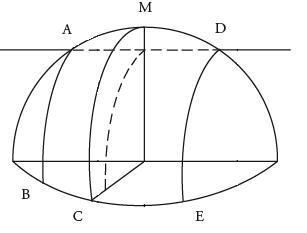
\includegraphics{repslatex-img86.png}
\end{marginfigure}

La proyección ordinaria es la de Gauss o transversa de Mercator. En la
proyección Trasversa Universal de Mercator, el cilindro envolvente
sufre una reducción y se torna secante cortando al elipsoide según
dos líneas AB y DE de la figura XI.1; la línea MC representa el
meridiano. Los círculos menores paralelos al meridiano central
aparecen representados en su verdadera magnitud, no así el meridiano
central que aparecerá representado con la misma longitud que los
círculos menores, es decir se reduce.

\ \ Sobre los círculos menores de sedancia el módulo de
deformación o factor de escala es igual a la unidad; en el meridiano
central será un valor menor que uno. Al módulo de deformación en
el meridiano central se lo denomina factor de reducción de escala.

\ \ En el sistema UTM el factor de escala en el meridiano central se
establece como:

\ \  ${k_{{0}}=1-\frac{1}{\text{2500}}=0\text{.}\text{9996}}$  (XI.1)

Es decir, los valores de las distancias medidas sobre el meridiano
aparecen reducidas según  ${k_{{0}}}$.

\ \ Este factor de escala equivale a ubicar los círculos menores de
sedancia en una longitud de 1{\textordmasculine} 37{\textquoteright}
14{\textquoteright}{\textquoteright} a ambos lados del meridiano
central. Sobre esas líneas el factor de escala se hace igual a uno y
más allá de ellas supera este valor.



\begin{marginfigure}
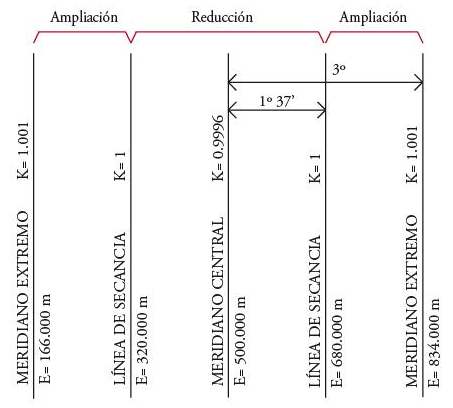
\includegraphics{repslatex-img87.png}
\end{marginfigure}

\ \ En la figura XI.2 se ilustra lo anterior. Existen dos zonas: una de
ampliación y otra de reducción.

\ \ En el sistema UTM los husos son de 6{\textordmasculine} de amplitud,
3{\textordmasculine} a cada lado del meridiano central. La ampliación
de la faja meridiana respecto de Gauss-Kruger, se hace compatible con
los módulos de deformación en los extremos por haber introducido en
el meridiano central el factor de reducción  ${k_{{0}}}$.

\ \ Las líneas de tangencia se encuentran situadas a unos 180 km a
ambos lados del meridiano central, y los meridianos extremos a unos 334
km. 

\ \ Las fajas de 6{\textordmasculine} de amplitud están limitados por
los meridianos múltiplos de 6{\textordmasculine} coincidiendo con los
husos de la carta mundial al millonésimo.

Cada sistema debe ser prolongado 30{\textquoteright} sobre los
contiguos, es decir los puntos pertenecientes a cada faja tienen
coordenadas en la propia y en la contigua, creándose así una zona
de superposición de 1{\textordmasculine} de ancho.

No son usadas las letras {\textquotedblleft}X{\textquotedblright} e
{\textquotedblleft}Y{\textquotedblright} para designar las coordenadas,
sino {\textquotedblleft}N{\textquotedblright} (norte) y
{\textquotedblleft}E{\textquotedblright} (este).

El origen de coordenadas planas en cada huso es el cruce del ecuador con
el meridiano central. La coordenada
{\textquotedblleft}N{\textquotedblright} se mide a partir del ecuador
pero para el hemisferio sur se las aumenta en 10.000.000 m evitando
valores negativos.

La coordenada {\textquotedblleft}E{\textquotedblright} se mide a partir
del meridiano central, positiva al Este y negativa al Oeste. Para
evitar valores negativos de {\textquotedblleft}E{\textquotedblright} se
adjudica al meridiano central la coordenada 500.000 m.

El número de faja es el mismo que en la Carta Internacional al
millonésimo, ésto es de 1 a 60 a contar del antimeridiano de
Greenwich.

El meridiano central de 177{\textordmasculine} (W) es la zona 1, el
171{\textordmasculine} (W) la zona 2 y así cada 6{\textordmasculine}.

La coordenada {\textquotedblleft}E{\textquotedblright} para las líneas
de sedancia son de acuerdo a lo anterior son 680.000 m y 320.000 m al
este y al oeste del meridiano central respectivamente; y las
coordenadas de los meridianos de borde de faja son 834.000 m y 166.000
m al este y al oeste.

Las correspondencias entre los números de zona de las coordenadas UTM
y el número de fajas de proyección Gauss-Kruger en la República
Argentina de acuerdo a las convenciones adoptadas son:

\begin{center}
\tablehead{}
\begin{supertabular}{|m{3.457cm}|m{2.351cm}|m{3.448cm}|}
\hline
\centering Meridiano Central &
\centering Zona UTM &
\centering\arraybslash Faja Gauss-Kruger\\\hline
\centering {}-51{\textordmasculine} &
\centering 22 &
\centering\arraybslash {}-\\\hline
\centering {}-54{\textordmasculine} &
 &
\centering\arraybslash 7\\\hline
\centering {}-57{\textordmasculine} &
\centering 21 &
\centering\arraybslash 6\\\hline
\centering {}-60{\textordmasculine} &
 &
\centering\arraybslash 5\\\hline
\centering {}-63{\textordmasculine} &
\centering 20 &
\centering\arraybslash 4\\\hline
\centering {}-66{\textordmasculine} &
 &
\centering\arraybslash 3\\\hline
\centering {}-69{\textordmasculine} &
\centering 19 &
\centering\arraybslash 2\\\hline
\centering {}-72{\textordmasculine} &
 &
\centering\arraybslash 1\\\hline
\centering {}-75{\textordmasculine} &
\centering 18 &
\centering\arraybslash {}-\\\hline
\end{supertabular}
\end{center}
\ \ En el sistema UTM el número de zona puede determinarse por medio
de la siguiente expresión:

 ${\normalsubformula{\text{ZONA}}=\frac{\left(\text{183}+\lambda
_{{0}}\right)}{6}}$\ \   (XI.2)

Donde  ${\lambda _{{0}}}$ es la longitud del meridiano central y se debe
introducir con su signo.

\ \ El número de faja de la proyección Gauss-Kruger para el
territorio argentino se puede encontrar por medio de:

\ \  ${\normalsubformula{\text{FAJA}}=\frac{\left(\text{75}+\lambda
_{{0}}\right)}{3}}$  (XI.3)

XI.2.- TRANSFORMACIÓN DE COORDENADAS GEOGRÁFICAS EN PLANAS.

\ \ El planteo de las expresiones de las coordenadas UTM es similar al
de las Gauss-Kruger, y es a través de las funciones de variable
compleja:

\ \ 
${x+\normalsubformula{\text{iy}}=f\left(q+\normalsubformula{\text{il}}\right)}$
 (XI.4)

Considerando puntos en el meridiano central

\begin{equation*}
{x=f\left(q\right)=B}
\end{equation*}
Donde {\textquotedblleft}B{\textquotedblright} es el arco de meridiano
elipsóidico que va del ecuador hasta la latitud considerada como se
determinó en la expresión (VIII.12).

\ \ Se desarrolla en serie de Taylor tomando
{\textquotedblleft}l{\textquotedblright} como incremento de la misma
forma que en la proyección Gauss-Kruger determinándose expresiones
similares con la diferencia que en el meridiano central se cuentan las
coordenadas a partir del ecuador.

\ \ Pero para reducir las deformaciones y poder ampliar las zonas, se
afectó al meridiano central según un factor de reducción 
${k_{{0}}}$, de manera tal que las distancias sobre el meridiano
central aparecen reducidas por el factor de escala, es decir que el
arco de meridiano del ecuador a la latitud en consideración habrá
que afectarlo por este factor

\ \  ${f\left(q\right)=k_{{0}}\cdot B}$  (XI.5)

la imagen geométrica de la proyección con este artificio del factor
de escala, se obtiene considerando un cilindro secante en lugar de
tangente según dos líneas que se representan en su verdadera
magnitud. En lugar de una línea sin deformación se obtienen dos,
simétricas respecto del meridiano central.

\ \ Las expresiones de las coordenadas UTM son similares a las de Gauss
con las siguientes modificaciones:

\begin{equation*}
{N=k_{{0}}\cdot [B+\frac{l^{{2}}\cdot \text{cos}^{{2}}\left(\varphi
\right)\cdot N\cdot t}{2}+\frac{l^{{4}}\cdot
\text{cos}^{{4}}\left(\varphi \right)\cdot N\cdot t\cdot
\left(5-t^{{2}}+9\cdot n^{{2}}+4\cdot n^{{4}}\right)}{\text{24}}+}
\end{equation*}
 ${+{\frac{l^{{6}}\cdot \text{cos}^{{6}}\left(\varphi \right)\cdot
N\cdot t\cdot \left(\text{61}-\text{58}\cdot
t^{{2}}+t^{{4}}+\text{270}\cdot n^{{2}}-\text{330}\cdot t^{{2}}\cdot
n^{{2}}\right)}{\text{720}}}]}$  (XI.6.a)

\begin{equation*}
{E=\text{500}\text{.}\text{000}+k_{{0}}\cdot [l\cdot
\text{cos}\left(\varphi \right)\cdot N+\frac{l^{{3}}\cdot
\text{cos}^{{3}}\left(\varphi \right)\cdot N\cdot t\cdot
\left(1-t^{{2}}+n^{{2}}\right)}{6}+}
\end{equation*}
 ${+{\frac{l^{{5}}\cdot \text{cos}^{{5}}\left(\varphi \right)\cdot
N\cdot t\cdot \left(5-\text{18}\cdot t^{{2}}+t^{{4}}+\text{14}\cdot
n^{{2}}-\text{58}\cdot t^{{2}}\cdot n^{{2}}\right)}{\text{120}}}]}$ 
(XI.6.b)

En el hemisferio sur se le suma la cantidad de 10.000.000 m a la
coordenada {\textquotedblleft}N{\textquotedblright}.

\ \ En el problema recíproco, es decir la transformación de
coordenadas planas a geográficas se computarán con las mismas
expresiones que las de Gauss-Kruger con la diferencia de que el valor
de {\textquotedblleft}y{\textquotedblright} se tomará como:

\ \  ${y=\frac{\left(E-\text{500}\text{.}\text{000}\right)}{k_{{0}}}}$ 
(XI.7)

Este mismo valor de {\textquotedblleft}y{\textquotedblright} se
adoptará para el círculo de la convergencia meridiana en la
expresión (X.28.b).

\ \ El módulo de deformación lineal se calculará introduciendo el
valor de  ${k_{{0}}}$:

\ \  ${m=k_{{0}}\cdot \left(1+\frac{y^{{2}}}{2\cdot
R^{{2}}}+\frac{y^{{4}}}{\text{24}\cdot R^{{4}}}\right)}$  (XI.8)

En cuanto a la deformación de distintas finitas la consideración es
la misma de modo que:

\ \  ${\frac{l}{L}=k_{{0}}\cdot \left(1+\frac{y_{{1}}^{{2}}+y^{{1}}\cdot
y^{{2}}+y_{{2}}^{{2}}}{6\cdot R^{{2}}}\right)}$  (XI.9)

\ \ La corrección el arco a la cuerda se obtiene de las (X.41.a) o
(X.41.b) pero teniendo en cuenta la (XI.7) en las (XI.8) y (XI.9);
también se introduce el valor de
{\textquotedblleft}y{\textquotedblright} de la (XI.7).

XI.3.- UNA EXPRESIÓN PARA AMBAS PROYECCIONES.

\ \ En las siguientes expresiones se debe tener en cuenta el signo de la
latitud y longitud, y son válidas para el hemisferio sur.

\begin{equation*}
{X=Q+k_{{0}}\cdot [B+\frac{l^{{2}}\cdot \text{cos}^{{2}}\left(\varphi
\right)\cdot N\cdot t}{2}+\frac{l^{{4}}\cdot
\text{cos}^{{4}}\left(\varphi \right)\cdot N\cdot t\cdot
\left(5-t^{{2}}+9\cdot n^{{2}}+4\cdot n^{{4}}\right)}{\text{24}}+}
\end{equation*}
 ${+{\frac{l^{{6}}\cdot \text{cos}^{{6}}\left(\varphi \right)\cdot
N\cdot t\cdot \left(\text{61}-\text{58}\cdot
t^{{2}}+t^{{4}}+\text{270}\cdot n^{{2}}-\text{330}\cdot t^{{2}}\cdot
n^{{2}}\right)}{\text{720}}}]}$  (XI.10.a)

\begin{equation*}
{Y=F+\text{500}\text{.}\text{000}+k_{{0}}\cdot [l\cdot
\text{cos}\left(\varphi \right)\cdot N+\frac{l^{{3}}\cdot
\text{cos}^{{3}}\left(\varphi \right)\cdot N\cdot t\cdot
\left(1-t^{{2}}+n^{{2}}\right)}{6}+}
\end{equation*}
 ${+{\frac{l^{{5}}\cdot \text{cos}^{{5}}\left(\varphi \right)\cdot
N\cdot t\cdot \left(5-\text{18}\cdot t^{{2}}+t^{{4}}+\text{14}\cdot
n^{{2}}-\text{58}\cdot t^{{2}}\cdot n^{{2}}\right)}{\text{120}}}]}$ 
(XI.10.b)

Donde:

\begin{equation*}
{t=\normalsubformula{\text{tg}}\left(\varphi \right)}
\end{equation*}
\begin{equation*}
{n^{{2}}=e'^{{2}}\cdot \text{cos}^{{2}}\left(\varphi \right)}
\end{equation*}
\begin{equation*}
{e'^{{2}}=\frac{a^{{2}}-b^{{2}}}{b^{{2}}}}
\end{equation*}
\begin{equation*}
{N=\frac{a}{\left[1-e^{{2}}\cdot
\normalsubformula{\text{sen}}^{{2}}\left(\varphi
\right)\right]^{{1/2}}}}
\end{equation*}
\ \ \ \  ${l=\lambda -\lambda _{{0}}}$  (expresada en radianes)

 ${\lambda _{{0}}}$ es la longitud del meridiano central de la faja
Gauss-Kruger o zona UTM en la que se proyectan los puntos.

{\textquotedblleft}B{\textquotedblright} es el arco de meridiano desde
el ecuador hasta la latitud considerada, por la expresión (VIII.12).

\begin{equation*}
{B=\alpha \cdot \varphi +\beta \cdot
\normalsubformula{\text{sen}}\left(2\cdot \varphi \right)+\gamma \cdot
\normalsubformula{\text{sen}}\left(4\cdot \varphi \right)+\delta \cdot
\normalsubformula{\text{sen}}\left(6\cdot \varphi \right)+\varepsilon
\cdot \normalsubformula{\text{sen}}\left(8\cdot \varphi \right)}
\end{equation*}
\ \ En el caso de Gauss-Kruger la coordenada por el meridiano central se
mide a partir del polo sur; para que ésto se cumpla en la expresión
(XI.10.a) se hace:

\begin{equation*}
{Q=\frac{a\cdot \pi }{2}}
\end{equation*}
En el caso de coordenadas UTM para el hemisferio sur, por lo
anteriormente visto, se tiene que:

\begin{equation*}
{Q=\text{10}\text{.}\text{000}\text{.}\text{000}m}
\end{equation*}
El factor de escala:

\ \  ${k_{{0}}=1}$\ \ \ \ \ \ (Gauss-Kruger)  

\ \  ${k_{{0}}=0\text{.}\text{9996}}$\ \ \ \ (U.T.M.)

{\textquotedblleft}F{\textquotedblright} se refiere al número de faja,
introducido en los millones de la coordenada
{\textquotedblleft}Y{\textquotedblright}

\ \  ${F=\left[\frac{\left(\text{75}+\lambda
_{{0}}\right)}{3}\right]\cdot \text{10}^{{6}}}$\ \ \ \ (Gauss-Kruger)

\ \  ${F=0}$\ \ \ \ \ \ \ \ (U.T.M.)

\ \ En la proyección UTM debe agregarse como información el valor de
la zona, ésto  es:

\begin{equation*}
{\normalsubformula{\text{ZONA}}=\frac{\text{183}+\lambda _{{0}}}{6}}
\end{equation*}
\ \ En la proyección Gauss-Kruger, los resultados de las coordenadas
(XI.10.a) y (XI.10.b) se expresan como
{\textquotedblleft}X{\textquotedblright} e
{\textquotedblleft}Y{\textquotedblright}. En el sistema UTM como
{\textquotedblleft}N{\textquotedblright} en lugar de
{\textquotedblleft}X{\textquotedblright}, y
{\textquotedblleft}E{\textquotedblright} en lugar de
{\textquotedblleft}Y{\textquotedblright}.

\ \ En ambas proyecciones, para la transformación son necesarias como
datos la latitud y longitud de los puntos con cuatro decimales, los
parámetros del elipsoide de referencia, longitud del meridiano
central.

\ \ En la transformación de coordenadas planas en coordenadas
geográficas se puede escribir:

\begin{equation*}
{\varphi =\varphi _{{1}}-\frac{y^{{2}}}{2\cdot M_{{1}}\cdot
N_{{1}}}\cdot t_{{1}}\cdot \left[1-\frac{y^{{2}}}{\text{12}\cdot
N_{{1}}^{{2}}}\cdot \left(5+3\cdot t_{{1}}^{{2}}+n_{{1}}^{{2}}-9\cdot
t_{{1}}^{{2}}\cdot n_{{1}}^{{2}}\right)+\frac{y^{{4}}}{\text{360}\cdot
N_{{1}}^{{4}}}\cdot \left(\text{61}+\text{90}\cdot
t_{{1}}^{{2}}+\text{45}\cdot t_{{1}}^{{4}}\right)\right]}
\end{equation*}
(XI.11.a)

\begin{equation*}
{\lambda =\lambda _{{0}}+\frac{y}{N_{{1}}\cdot \text{cos}\left(\varphi
_{{1}}\right)}\cdot \left[1-\frac{y^{{2}}}{6\cdot N_{{1}}^{{2}}}\cdot
\left(1+2\cdot
t_{{1}}^{{2}}+n_{{1}}^{{2}}\right)+\frac{y^{{4}}}{\text{120}\cdot
N_{{1}}^{{4}}}\cdot \left(5+\text{28}\cdot t_{{1}}^{{2}}+\text{24}\cdot
t_{{1}}^{{4}}+6\cdot n_{{1}}^{{2}}-8\cdot n_{{1}}^{{2}}\cdot
t_{{1}}^{{2}}\right)\right]}
\end{equation*}
(XI.11.b)

Donde:

\begin{equation*}
{M=\frac{a\cdot \left(1-e^{{2}}\right)}{\left[1-e^{{2}}\cdot
\normalsubformula{\text{sen}}^{{2}}\left(\varphi
\right)\right]^{{3/2}}}}
\end{equation*}
\begin{equation*}
{y=\frac{\left(Y-F-\text{500}\text{.}\text{000}\right)}{k_{{0}}}}
\end{equation*}
\ \ 
${\normalsubformula{\text{NF}}=\frac{F}{\text{10}^{{6}}}}$\ \ \ \ \ \ (número
de faja en Gauss-Kruger)

\ \  ${\lambda _{{0}}=3\cdot
\normalsubformula{\text{NF}}-\text{75}}$\ \ \ \ (para Gauss-Kruger)

\ \  ${\lambda _{{0}}=6\cdot
\normalsubformula{\text{ZONA}}-\text{183}}$\ \ \ \ (para UTM)

es el arco de meridiano correspondiente a
{\textquotedblleft}x{\textquotedblright} siendo:

\begin{equation*}
{x=\frac{X-Q}{k_{{0}}}}
\end{equation*}
\ \  ${Q=\frac{\alpha \cdot \pi }{2}}$\ \ \ \ \ \ (para Gauss-Kruger)

\ \  ${Q=\text{10}\text{.}\text{000}\text{.}\text{000}m}$\ \ \ \ (para
UTM)

El valor de  ${\varphi _{{1}}}$ se halla con las aproximaciones
sucesivas vistas en (X.3).

\ \ Los resultados de las (XI.11) están expresados en radianes; notar
que tanto  ${\varphi _{{1}}}$ y  ${\lambda _{{0}}}$ deben ser
introducidos en radianes.

\ \ Para la transformación son necesarias como dato X o N, Y o E, los
parámetros del elipsoide de referencia.

\end{document}
